\documentclass[11pt]{article}\usepackage[T1]{fontenc}\usepackage[margin=.7in]{geometry}\usepackage{graphicx,booktabs,longtable,amsmath}\setlength{\parindent}{0pt}\begin{document}\section*{Original Continual World learners connected to OpenSim}
SMOKE: software integration only. Short10-step trajectories are intentionally truncated; they do not establish tracking quality, retention or CL benefit.
\begin{center}\small\begin{tabular}{llrrrrrr}\toprule Case & Method & Trials & Done & Failed & Trunc. & Passed & RMSE$^*$\\\midrule
A\_90 & no\_cl & 1 & 0 & 0 & 1 & 0 & --\\
A\_90 & packnet & 1 & 0 & 0 & 1 & 0 & --\\
B\_60 & no\_cl & 1 & 0 & 0 & 1 & 0 & --\\
B\_60 & packnet & 1 & 0 & 0 & 1 & 0 & --\\
C\_30 & no\_cl & 1 & 0 & 0 & 1 & 0 & --\\
C\_30 & packnet & 1 & 0 & 0 & 1 & 0 & --\\
D\_45 & no\_cl & 1 & 0 & 0 & 1 & 0 & --\\
D\_45 & packnet & 1 & 0 & 0 & 1 & 0 & --\\
\bottomrule\end{tabular}\end{center}
Completed-trial mean RMSE only; failed and truncated results have no invented final error.
\subsection*{What is unchanged}
Original source commit 73f63bb4fa0b5d00bda973e20dfb783bfcf1b8aa. SAC losses, target updates, actor/critic implementations, optimizers and PackNet pruning/gradient masks are imported directly from upstream/. All46 included upstream source/text files are Git-blob checksum verified before execution.
\subsection*{What is adapted}
The external environment adapter supplies OpenSim states, a force action, tracking reward, resets, episode limits and success criteria. A32-dimensional observation contains28 encoded physical/reference/muscle features plus a4-dimensional known-case selector. With hide\_task\_id=True the shared core uses28 inputs; the selector chooses the appropriate output head. The action a in[-1,1] maps to F=325(a+1)N. Shoulder/yaw and5kg load follow the original scenarios; muscle strengths are A90\%,B60\%,C30\%,D45\%.
\subsection*{Learning architecture and budgets}
Four256-neuron hidden layers, leaky-ReLU with first-layer normalization/tanh as in upstream, four policy heads, two critics and target critics. The full configuration uses1M environment steps per case, batch128, Adam0.001, gamma0.99, automatic entropy with target output std0.089, FIFO replay1M and reset at case boundaries. No CL means SAC fine-tuning; SAC still uses within-case replay. PackNet additionally uses100k pruning/retraining updates per nonfinal case and clipnorm2e-5, following the authors paper command. It therefore has additional compute. Equal budgets mean new simulator steps, not total gradient updates.
\subsection*{Reward definition}
At each control step: exp(-(angle\_error\_deg/5)^2) -0.01(F/650)^2 -0.01(deltaF/650)^2 -0.05 min((velocity\_error\_rad\_s/0.5)^2,25). Physical failure reward=-20. These are task-specific adapter choices, not equations claimed from the paper. Settings are fixed before final tests.
\subsection*{Physical and evaluation limits}
Control interval0.02s, integrator maximum step0.005s, real OpenSim dynamics with the original model. Requested force is bounded0..650N; elbow3..123deg and positive cable moment arm are checked. A completed reference passes when motion-only RMSE<=0.5deg and peak<=2deg. Full peak and failures are retained. Time-limit truncation is separate from physical failure. The worker never returns a fabricated successful transition after an infrastructure exception.
\subsection*{Data split and fairness}
420 configurations for interaction training,60 for periodic validation and120 reserved for final frozen evaluation. The paired final evaluations use the same reference IDs. On-policy trajectories and the number of episodes need not match between methods. Actor initial-weight fingerprints are checked for equality across methods. Seed42 only; episode diversity is not independent training replication. No candidate or checkpoint is chosen using reserved tests.
\subsection*{Interpretation limits}
A complete run is not proof of good tracking or CL superiority. This first comparison does not measure forward transfer because independent single-case reference training runs have not been included. It is not an offline600-episode supervised experiment and does not reproduce the authors robotic benchmark scores.
\subsection*{Saved models and recovery}
Original actor/critic TensorFlow checkpoint prefixes and additional PackNet ownership state are retained. The unchanged upstream run loop cannot resume exactly in the middle of a method. Completed methods are reused by checksum; interrupted methods restart in a new attempt folder. Intermediate policies are deployable snapshots, not exact training-resume checkpoints.
\subsection*{Source and citation}
Wolczyk et al., Continual World: A Robotic Benchmark for Continual Reinforcement Learning, NeurIPS2021. https://github.com/awarelab/continual\_world. No upstream learning source is patched or reimplemented. Environment binding replaces continualworld.envs at import with only the OpenSim dimension constants; the original MuJoCo environment module is retained on disk but not imported.
\[J_Q=\mathbb{E}[(Q-y)^2],\quad J_\pi=\mathbb{E}[\alpha\log\pi(a|s)-\min(Q_1,Q_2)]\]
Original SAC objectives are imported, not rewritten. PackNet masks gradients and prunes/fixes parameter subsets; no replay-beta penalty is added for PackNet.
\clearpage\section*{Comparison}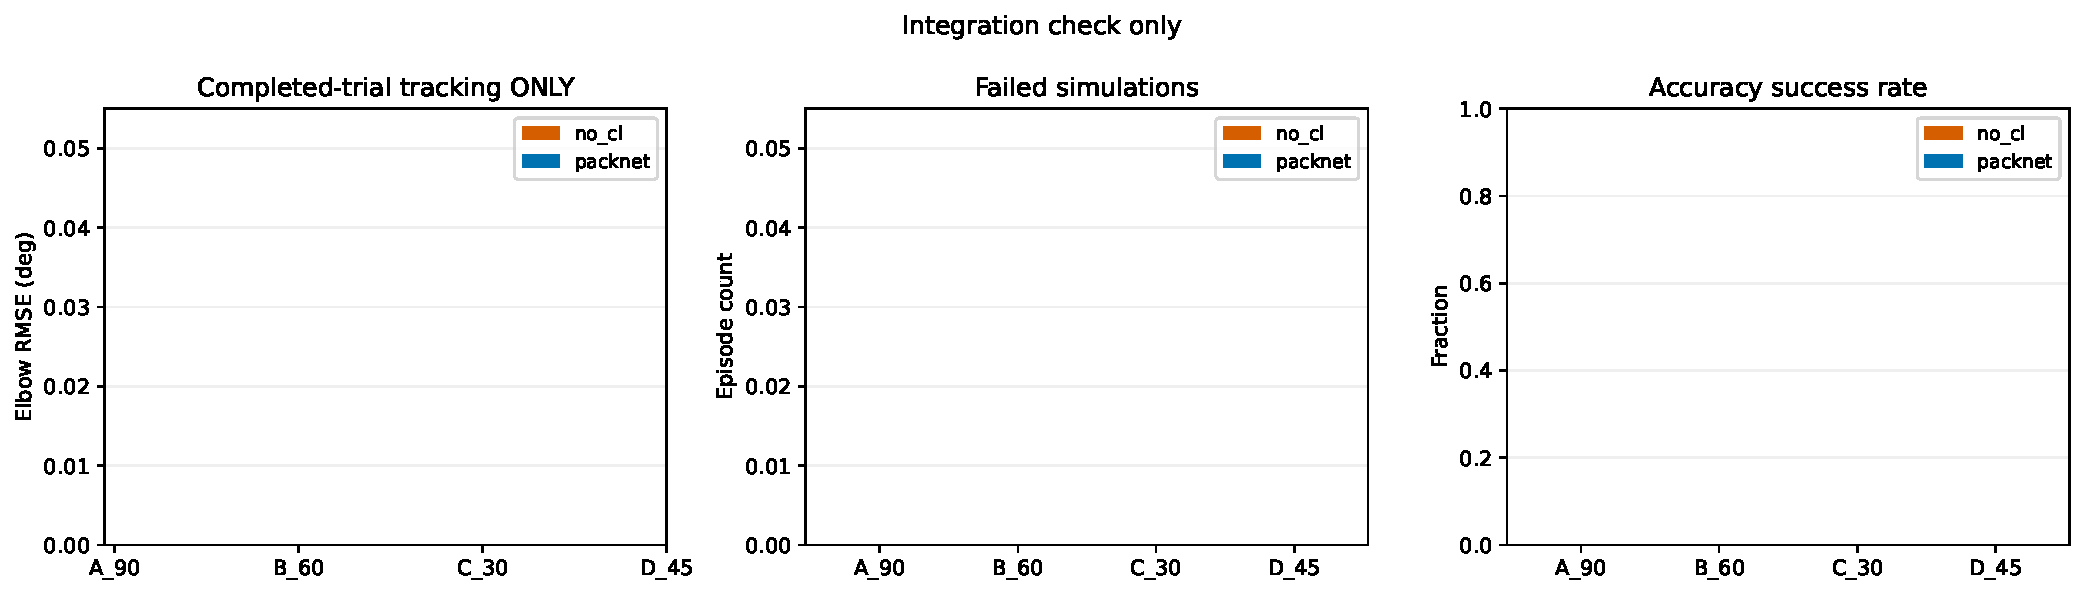
\includegraphics[width=\linewidth,height=.82\textheight,keepaspectratio]{figures/comparison.pdf}
\clearpage\section*{Learning}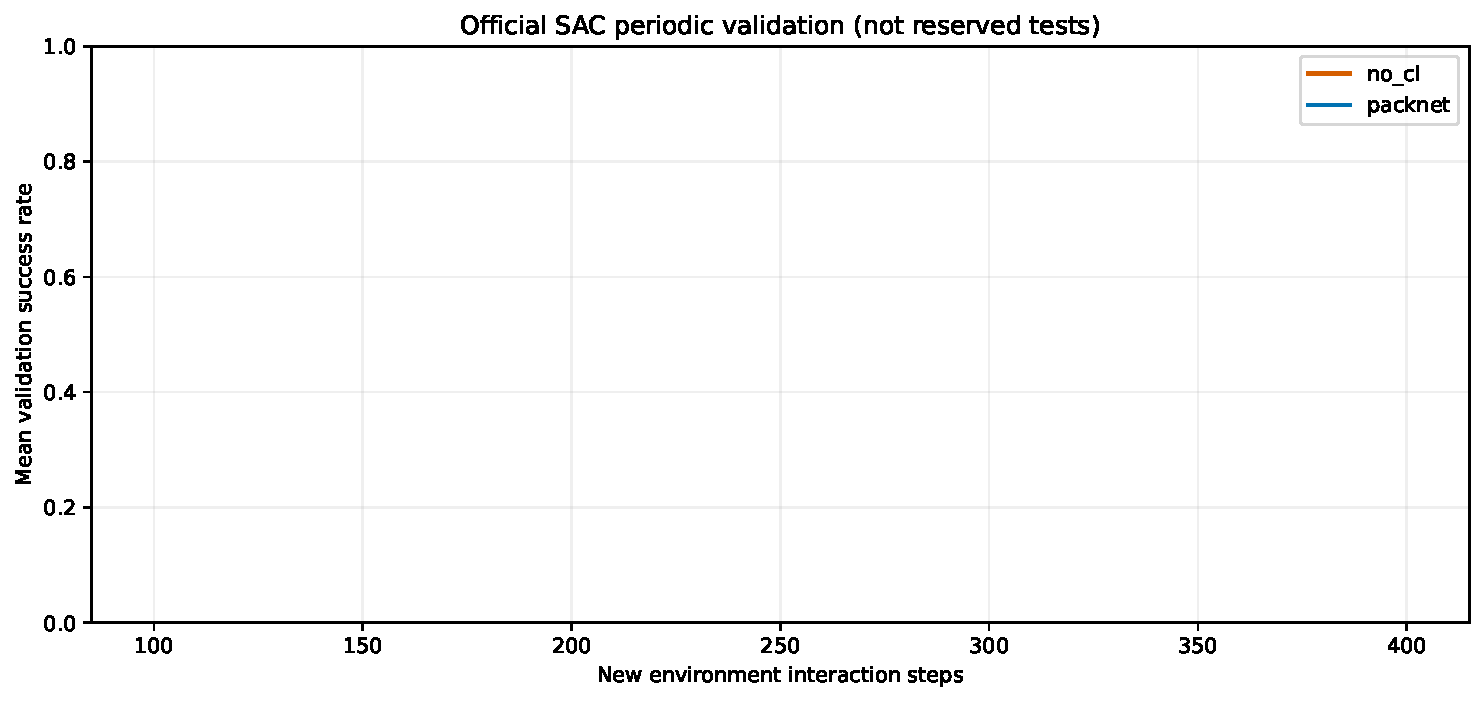
\includegraphics[width=\linewidth,height=.82\textheight,keepaspectratio]{figures/learning.pdf}
\clearpage\section*{Tracking A 90}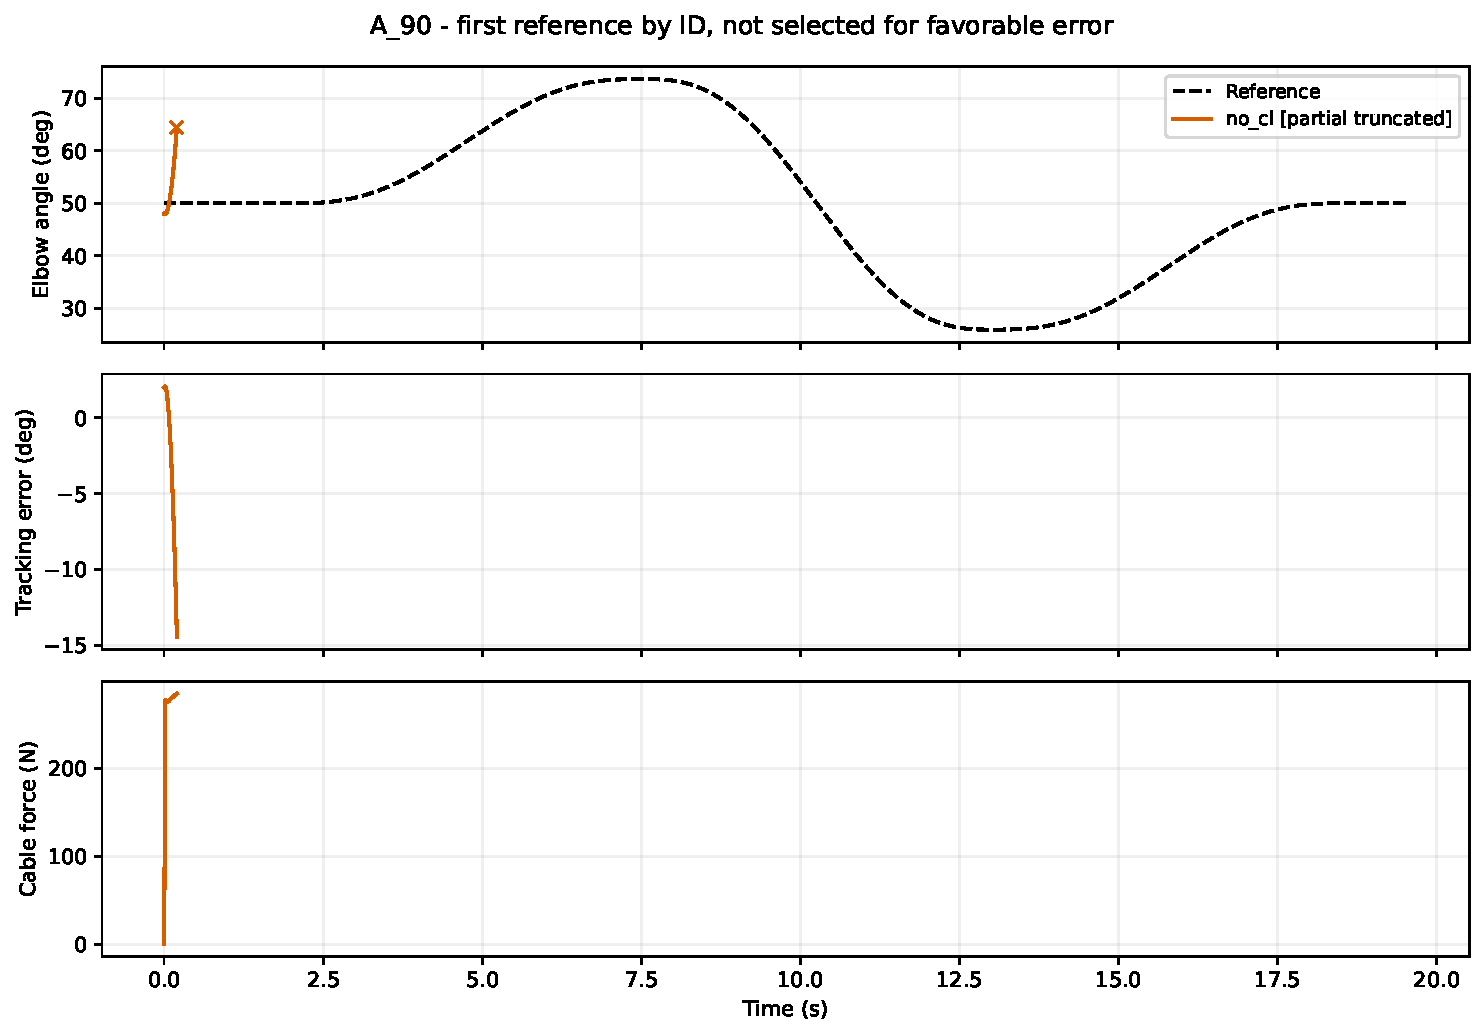
\includegraphics[width=\linewidth,height=.82\textheight,keepaspectratio]{figures/tracking_A_90.pdf}
\clearpage\section*{Tracking B 60}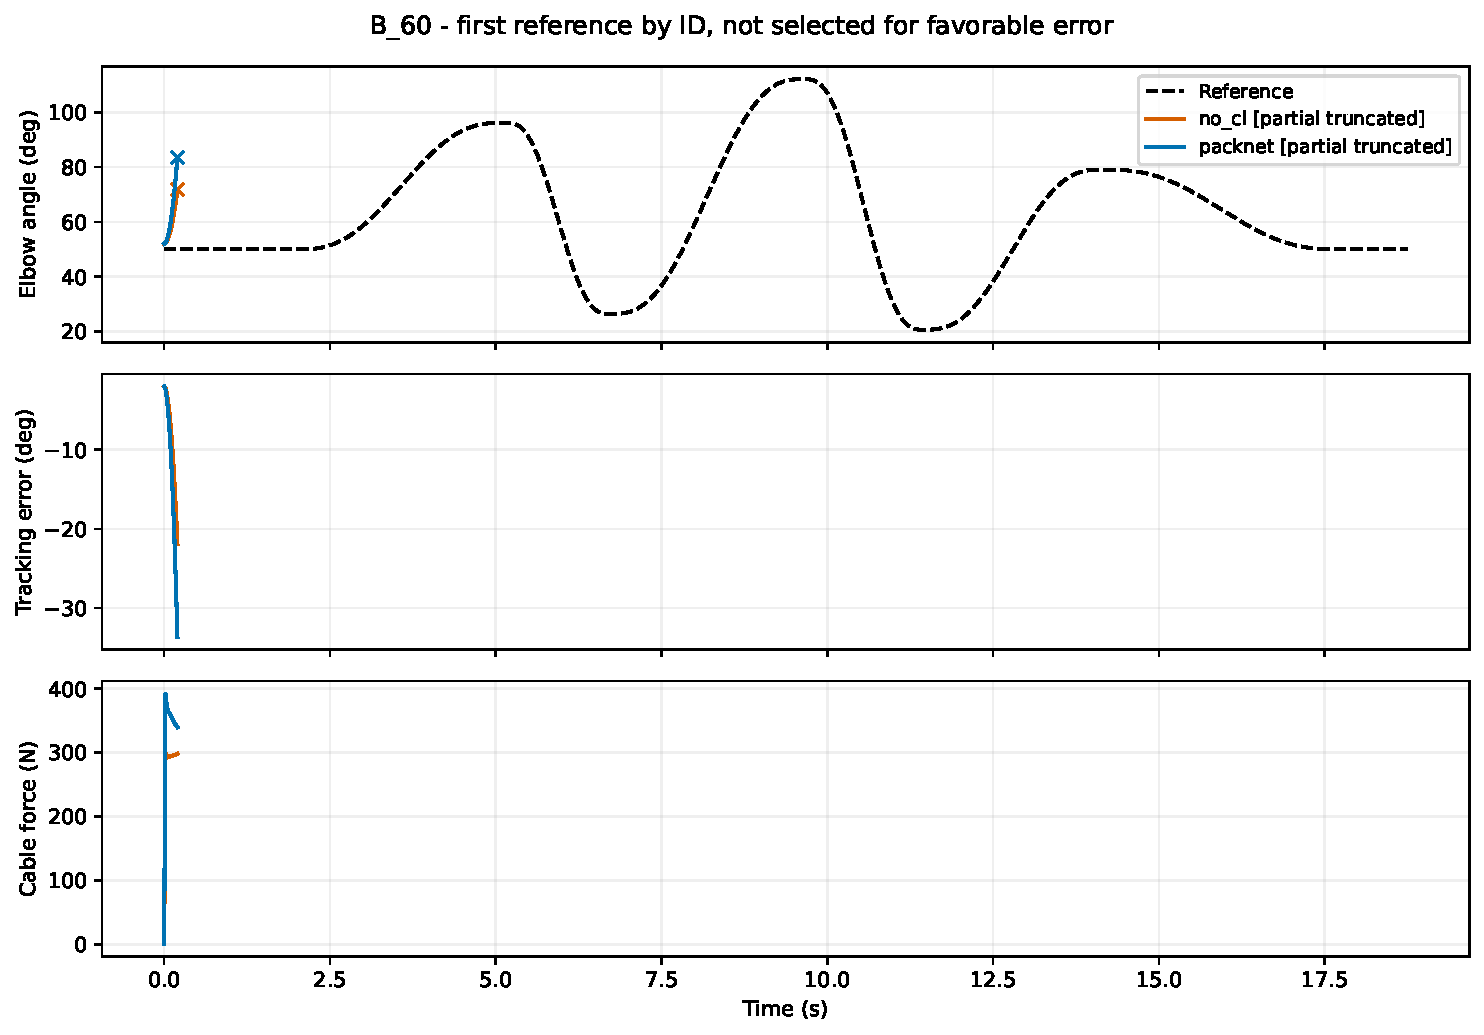
\includegraphics[width=\linewidth,height=.82\textheight,keepaspectratio]{figures/tracking_B_60.pdf}
\clearpage\section*{Tracking C 30}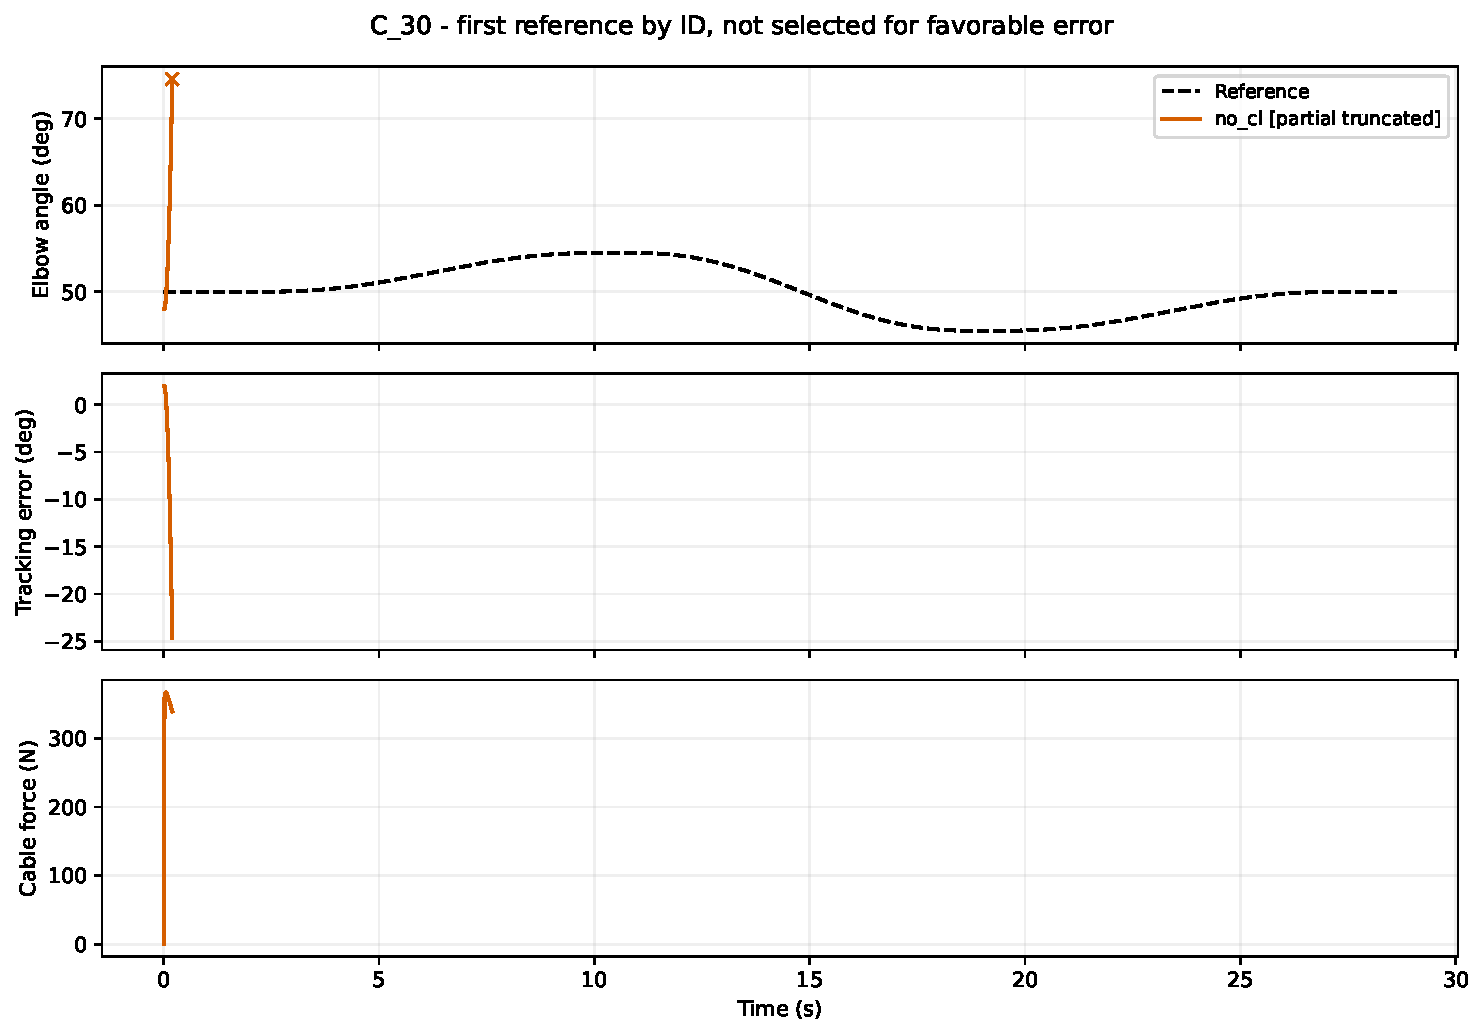
\includegraphics[width=\linewidth,height=.82\textheight,keepaspectratio]{figures/tracking_C_30.pdf}
\clearpage\section*{Tracking D 45}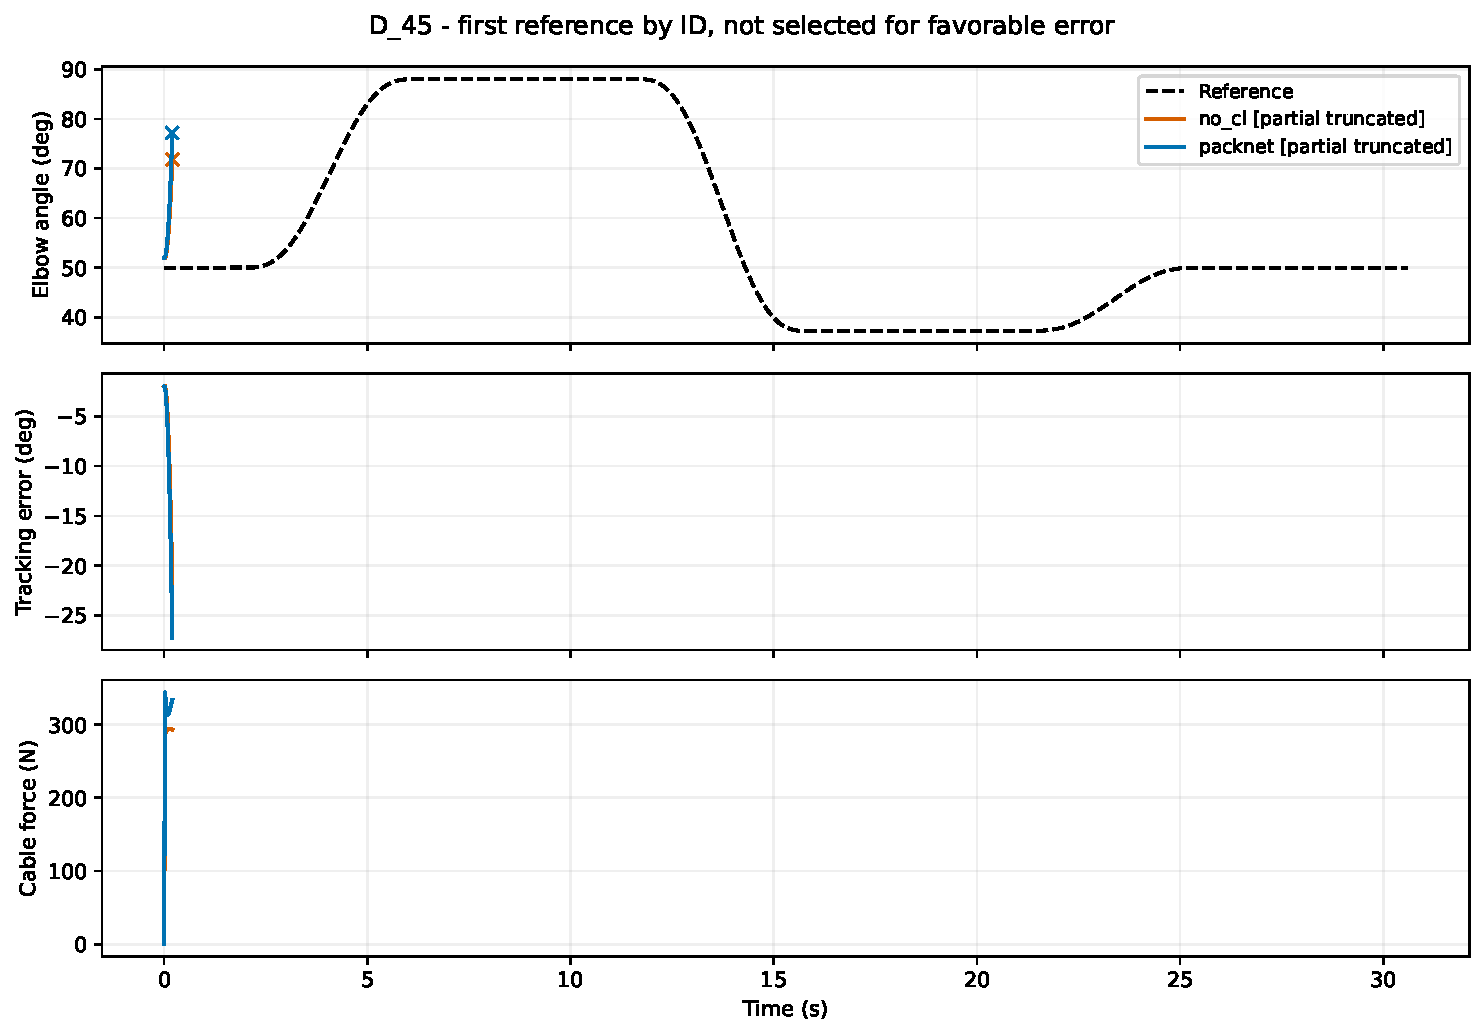
\includegraphics[width=\linewidth,height=.82\textheight,keepaspectratio]{figures/tracking_D_45.pdf}
\end{document}